\section{Pruning and Compression}\label{pruning}


Note that s is a quality parameter / sensitivity value according to the paper.
  According to Song Han's previous paper (Learning both Weights and Connections for Efficient Neural Networks),
  'The pruning threshold is chosen as a quality parameter multiplied by the standard deviation of a layer’s weights'
threshold = np.std(module.weight.data.cpu().numpy()) * s

\begin{table*}[!htb]
\begin{center}
\renewcommand\arraystretch{1.5}
\fontsize{6.7pt}{6.7pt}\selectfont
\begin{tabular}{|c|c|c|c|c|c|c|c|}
\hline
\multicolumn{8}{|c|}{\textbf{FashionMNIST Dataset}}\\
\multicolumn{2}{|c}{\textbf{Baseline Model =>}} & \multicolumn{2}{c}{\textbf{Train Accuracy:} 98.64\%} & \multicolumn{2}{c}{\textbf{Test Accuracy:} 89.66\%} & \multicolumn{2}{c|}{\textbf{Inference Accuracy:} 55.26\%}\\
\hline
\multirow{3}{*}{\textbf{Sensitivity}} & \multicolumn{4}{|c|}{On Pruning} & \multicolumn{3}{|c|}{Retraining}\\
\hline
 & \textbf{Train}  & \textbf{Test}  & \textbf{Inference}  & \textbf{Compression} & \textbf{Train}  & \textbf{Test}  & \textbf{Inference}  \\
                      & \textbf{Accuracy} & \textbf{Accuracy} & \textbf{Accuracy} & \textbf{Rate} & \textbf{Accuracy} & \textbf{Accuracy} & \textbf{Accuracy}  \\

\hline
0.25 & 98.58\% & 89.47\% & \cellcolor{green!25}55.18\% & 1.35x & 99.47\% & 89.53\% & \cellcolor{red!25}55.61\%\\
0.5 & 97.78\% & 89.17\% & \cellcolor{green!25}54.87\% & 1.87x & 99.56\% & 90.00\% & \cellcolor{red!25}55.82\%\\
0.75 & 94.97\% & 87.43\% & \cellcolor{green!25}53.86\% & 2.63x & 99.66\% & 89.56\% & \cellcolor{red!25}55.91\%\\
1 & 90.31\% & 84.45\% & \cellcolor{green!25}53.18\% & 3.76x & 99.65\% & 89.76\% & \cellcolor{red!25}55.84\%\\
1.25 & 86.68\% & 81.8\% & \cellcolor{green!25}52.46\% & 5.40x & 99.85\% & 89.73\% & \cellcolor{red!25}56.04\%\\
1.5 & 69.12\% & 65.94\% & \cellcolor{green!25}51.77\% & 7.80x & 99.75\% & 89.47\% & \cellcolor{red!25}56.04\%\\
1.75 & 49.24\% & 47.35\% & \cellcolor{green!25}51.40\% & 11.20x & 99.77\% & 89.01\% & \cellcolor{red!25}56.20\%\\
2 & 31.69\% & 30.38\% & \cellcolor{green!25}50.82\% & 15.95x & 99.89\% & 88.38\% & \cellcolor{red!25}56.69\%\\
\hline
\hline
\multicolumn{8}{|c|}{\textbf{Purchase Dataset}}\\
\multicolumn{2}{|c}{\textbf{Baseline Model =>}} & \multicolumn{2}{c}{\textbf{Train Accuracy:} 98.24\%} & \multicolumn{2}{c}{\textbf{Test Accuracy:} 88.22\%} & \multicolumn{2}{c|}{\textbf{Inference Accuracy:} 57.64\%}\\
\hline
0.25 & 98.20\% & 88.15\% & \cellcolor{green!25}57.62\% & 1.26x & 98.67\% & 87.95\% & \cellcolor{red!25}58.12\%\\
0.5 & 95.39\% & 85.37\% & \cellcolor{green!25}56.21\% & 1.65x & 99.12\% & 88.66\% & \cellcolor{red!25}58.52\%\\
0.75 & 84.78\% & 76.96\% & \cellcolor{green!25}54.04\% & 2.24x & 99.52\% & 88.94\% & \cellcolor{red!25}58.83\%\\
1 & 61.17\% & 58.04\% & \cellcolor{green!25}51.60\% & 3.13x & 99.74\% & 89.28\% & \cellcolor{red!25}59.01\%\\
1.25 & 41.22\% & 39.96\% & \cellcolor{green!25}50.81\% & 4.45x & 99.69\% & 88.51\% & \cellcolor{red!25}59.04\%\\
1.5 & 22.97\% & 22.78\% & \cellcolor{green!25}50.38\% & 6.37x & 99.89\% & 87.61\% & \cellcolor{red!25}59.71\%\\
1.75 & 15.72\% & 15.58\% & \cellcolor{green!25}50.34\% & 8.96x & 99.82\% & 85.28\% & \cellcolor{red!25}60.44\%\\
2 & 12.62\% & 12.20\% & \cellcolor{green!25}50.31\% & 12.10x & 99.64\% & 82.50\% & \cellcolor{red!25}61.05\%\\
\hline
\hline
\multicolumn{8}{|c|}{\textbf{Location Dataset}}\\
\multicolumn{2}{|c}{\textbf{Baseline Model =>}} & \multicolumn{2}{c}{\textbf{Train Accuracy:} 100.00\%} & \multicolumn{2}{c}{\textbf{Test Accuracy:} 62.3\%} & \multicolumn{2}{c|}{\textbf{Inference Accuracy:} 83.32\%}\\
\hline
0.5 & 100.00\% & 64.78\% & \cellcolor{green!25}82.54\% & 1.50x & 100\% & 64.61\% & \cellcolor{red!25}85.75\%\\
0.75 & 100.00\% & 62.70\% & \cellcolor{green!25}82.68\% & 1.94x & 100\% & 61.95\% & \cellcolor{red!25}87.69\%\\
1 & 99.96\% & 62.03\% & \cellcolor{green!25}78.76\% & 2.81x & 100\% & 62.43\% & \cellcolor{red!25}86.34\%\\
1.25 & 99.38\% & 60.39\% & \cellcolor{green!25}75.29\% & 3.43x & 100\% & 62.03\% & \cellcolor{red!25}85.25\%\\
1.5 & 95.60\% & 57.82\% & \cellcolor{green!25}70.98\% & 4.62x & 100\% & 61.15\% & \cellcolor{red!25}84.60\%\\
\hline
\end{tabular}
\end{center}
\caption{Privacy Risks for Pruning Neural Networks.}
\label{fmnist_pruning}
\end{table*}





\cite{45932}\cite{cap}
The capacity is measured using the mutual information, defined as a measure of the amount of information that one random variable contains about another random variable. The mutual information of a trained network with N input samples is calculated as follows:
\begin{equation}
I ( Y ; Y_{\theta}' | X ) = H ( Y | X ) - H ( Y | Y_{\theta}' , X )
\end{equation}
\begin{equation}
=N (1-(plog2 p+(1-p)log2 (1-p)) )
\end{equation}
where p is the mean classification accuracy for all samples under trained parameter theta. If the training accuracy is 1, the model memorizes all random samples and the I (Y ; Y' |X ) becomes the number
of samples N . If the training accuracy is 0.5, I (Y ; Y' |X ) goes to theta.
The accuracy, p, may vary depending on the training method of the model. We find N and p that maximize the mutual information of the networks by iteratively training the models.
X = \{$X_1,...,X_N$\},Xi $\in$ $(0,1)^{|N|}$
Y = $\{Y_1,...,Y_N\}$,$Y_i$ $\in$ (0,1),
Y' = $\{Y_1', ..., Y_N'\}, Y_i$' = f($\theta, X_i$),
where $f(\theta,X_i)$ is the predict of a network when the input is $X_i$. Under our experimental setting, both X and Y have uniform random distribution. Note that X and Y are independent as well as $Y_i$ and $Y_j$ when i not= j. Therefore
$P (Y_i|X_i) = P (Y_i) = 1/2$, and $H(Y) = H(Y_1, ..., Y_N ) = N H(Y_1) = N$.

And we use the network’s average accuracy p as a probability of Yi = Y'i, so that

\[
    P(Yi|Y'i)=
\begin{cases}
    p, & \text{if } Yi =Y'i\\
    (1 - p),  & \text{otherwise}
\end{cases}
\]

Finally, the equation is derived as:
\begin{equation}
I(Y;Y'|X)= H ( Y | X ) - H ( Y | Y' , X )
\end{equation}
\begin{equation}
= H ( Y ) - H ( Y | Y' ) = N -   H ( Y i | Y' i )
\end{equation}
\begin{equation}
= N -   H ( Y i | Y' i )
\end{equation}
\begin{equation}
=N-N plog2 p+(1-p)log2 (1-p)
\end{equation}
This captures
the amount of information stored in the parameters about the mapping between X and Y. To get an estimate of bits per parameter, we divide by the number of parameters,

\subsection{Sparsity vs Pruning}

We consider both the apporaches of sparsity and Pruning and evaluate their impact on membership privacy risks.
Sparsity zeros out the T\% of the parameters close to zero. In other words, the approach removes the frequently occurring parameters in the network, and forcing the model to train on the remaining network.
On the other hand, pruning ranks all the parameters and filters in a Neural Network and removes the unnecessary less occurring parameters in the network.
From the perspective of parameter distribution, pruning removes the parameters from the tail end of the distribution while sparsity removes the parameters closer to zero.

\begin{figure*}[ht!]
\begin{center}% note that \centering uses less vspace...
\resizebox{2\columnwidth}{!}{%
\begin{tabular}{lllll}


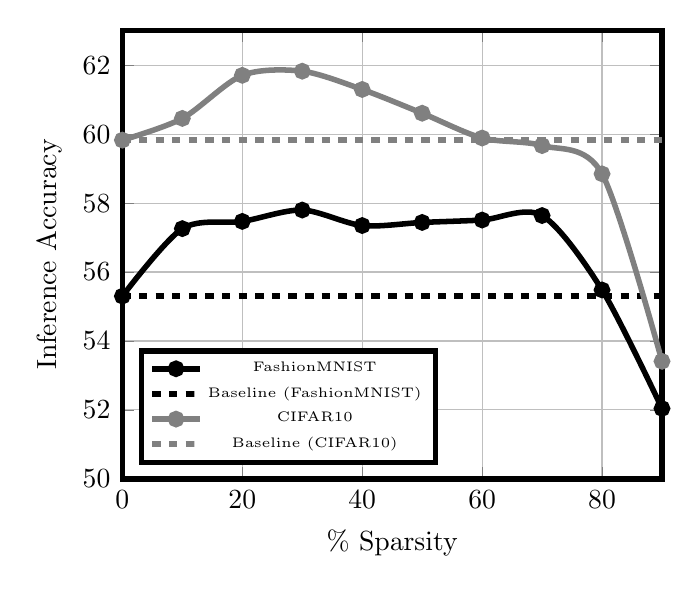
\begin{tikzpicture}
\begin{axis}[
legend style={font=\tiny},
legend pos =  south west,
line width=2.0pt,
mark size=2.0pt,
ymin=50,
xmin=0,
xmax=90,
legend entries={FashionMNIST, Baseline (FashionMNIST), CIFAR10, Baseline (CIFAR10)},
ylabel={Inference Accuracy},
xlabel={\% Sparsity},
% extra x ticks={1,10,...,400},
% extra y ticks={0,0.5,...,10},
% extra y tick labels={},
% extra x tick labels={},
% extra x tick style={grid=major},
% extra y tick style={grid=major},
grid=major
]
\addplot[
    color=black,
    solid,
    mark=*,
    mark options={solid},
    smooth
    ]
    coordinates {
    (0,55.30)(10,57.26)(20,57.47)(30,57.80)(40,57.35)(50,57.44)(60,57.51)(70,57.64)(80,55.48)(90,52.04)
      };
\addplot[
    color=black,
    dashed,
    smooth
    ]
    coordinates {
    (0,55.30)(10,55.30)(20,55.30)(30,55.30)(40,55.30)(50,55.30)(60,55.30)(70,55.30)(80,55.30)(90,55.30)
      };
\addplot[
    color=gray,
    solid,
    mark=*,
    mark options={solid},
    smooth
    ]
    coordinates {
    (0,59.83)(10,60.46)(20,61.71)(30,61.83)(40,61.30)(50,60.61)(60,59.89)(70,59.67)(80,58.85)(90,53.41)
      };
\addplot[
    color=gray,
    dashed,
    smooth
    ]
    coordinates {
    (0,59.83)(10,59.83)(20,59.83)(30,59.83)(40,59.83)(50,59.83)(60,59.83)(70,59.83)(80,59.83)(90,59.83)
      };
\end{axis}
\end{tikzpicture} &


%
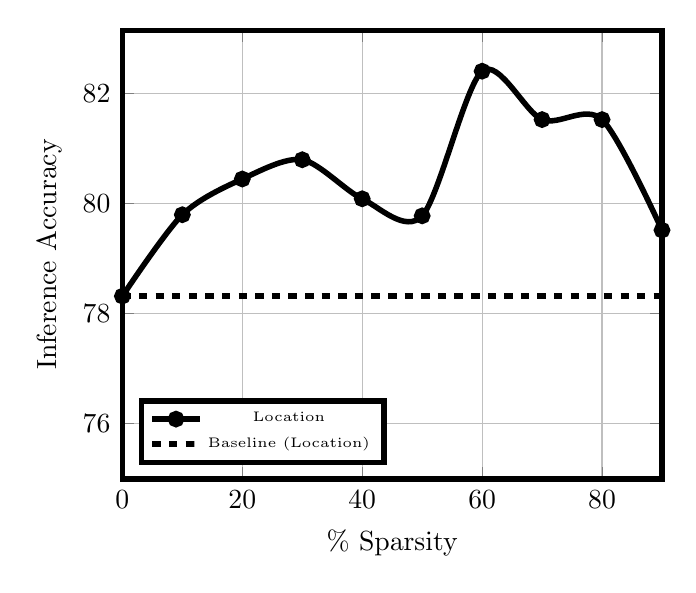
\begin{tikzpicture}
\begin{axis}[
legend style={font=\tiny},
legend pos =  south west,
line width=2.0pt,
mark size=2.0pt,
ymin=75,
xmin=0,
xmax=90,
legend entries={Location, Baseline (Location)},
ylabel={Inference Accuracy},
xlabel={\% Sparsity},
grid=major
]
\addplot[
    color=black,
    solid,
    mark=*,
    mark options={solid},
    smooth
    ]
    coordinates {
    (0,78.32)(10,79.80)(20,80.45)(30,80.80)(40,80.09)(50,79.78)(60,82.41)(70,81.53)(80,81.53)(90,79.52)
      };
\addplot[
    color=black,
    dashed,
    smooth
    ]
    coordinates {
    (0,78.32)(10,78.32)(20,78.32)(30,78.32)(40,78.32)(50,78.32)(60,78.32)(70,78.32)(80,78.32)(90,78.32)
      };

\end{axis}
\end{tikzpicture} &





%
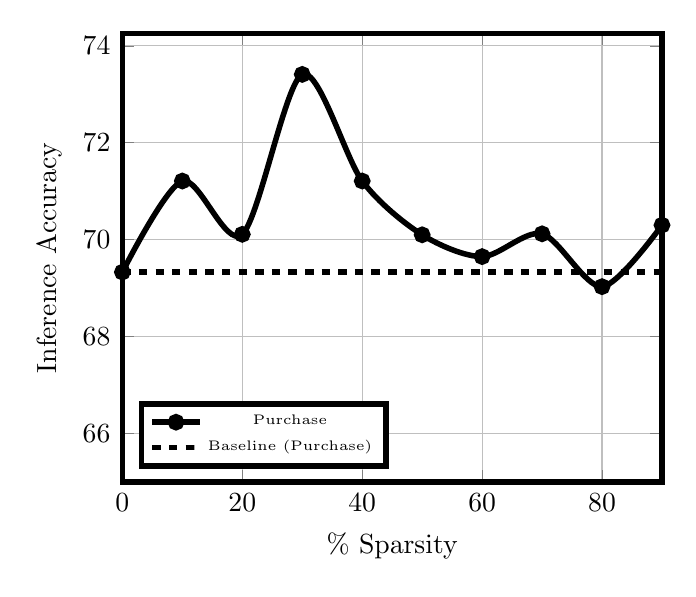
\begin{tikzpicture}
\begin{axis}[
legend style={font=\tiny},
legend pos =  south west,
line width=2.0pt,
mark size=2.0pt,
ymin=65,
xmin=0,
xmax=90,
legend entries={Purchase, Baseline (Purchase)},
ylabel={Inference Accuracy},
xlabel={\% Sparsity},
grid=major
]
\addplot[
    color=black,
    solid,
    mark=*,
    mark options={solid},
    smooth
    ]
    coordinates {
    (0,69.33)(10,71.21)(20,70.11)(30,73.41)(40,71.21)(50,70.10)(60,69.65)(70,70.12)(80,69.03)(90,70.30)
      };
\addplot[
    color=black,
    dashed,
    smooth
    ]
    coordinates {
    (0,69.33)(10,69.33)(20,69.33)(30,69.33)(40,69.33)(50,69.33)(60,69.33)(70,69.33)(80,69.33)(90,69.33)
      };

\end{axis}
\end{tikzpicture}


\end{tabular}
}
\caption{.}
\label{fig:loss}
\end{center}
\end{figure*}





\subsection{Pruning + Weight sharing}
DeepCompression
We evaluate the effectiveness of pruning followed by quantization which has been shown to have significant impact on reducing the model complexity through compression more significantly than either pruning or quantization alone.
We use the same model after pruning with Sensitivity since, it leaks the most information and evaluate the effective of quantization and whehter it can enable a good balance between test accuracy and inference accuracy.


\input{wtsharing_fig}
